\documentclass[12pt, letterpaper, twoside]{article}
\usepackage[T2A]{fontenc}	% поиск в PDF
\usepackage[english, russian]{babel}

\title{SmartCalc v1.0}
\author{justicer}

\usepackage{graphicx}
\graphicspath{ {images/} }

\newcommand{\code}[1]{\texttt{#1}}

\begin{document}
	
	\maketitle
	
	\section{Makefile}
	\begin{enumerate}
		\item Для установки SmartCalc v1.0 откройте терминал, перейдите в папку src и выполните команду: \code{make install} \par  Появится новая папка \verb|SmartCalcv_1.0|, в которой будет содержаться исполняемый файл для запуска. Чтобы запустить приложение выполните команду: \code{./SmartCalc}
		\item Для удаления SmartCalc v1.0 откройте терминал, перейдите в папку src и выполните команду: \code{make uninstall}
		\item Для архивации SmartCalc v1.0 откройте терминал, перейдите в папку src и выполните команду: \code{make dist}  \par  Появится архив \verb|Archive_SmartCalc_v1.0.tgz|
		\item Для открытия документации SmartCalc v1.0 откройте терминал, перейдите в папку src и выполните команду: \code{make dvi}
		\item Для удаления всех файлов и возврата к начальному состоянию SmartCalc v1.0 откройте терминал, перейдите в папку src и выполните команду: \code{make clean}
		\item Для проведения тестов SmartCalc v1.0 откройте терминал, перейдите в папку src и выполните команду: \code{make test}
		\item Для исследования покрытия кода тестами SmartCalc v1.0 откройте терминал, перейдите в папку src и выполните команду: \code{make gcov\textunderscore report}
		\item Для открытия отчета исследования покрытия кода тестами SmartCalc v1.0 после команды  \code{make gcov\textunderscore report}, выполните команду: \code{make open}
	\end{enumerate}

	\section{Calculator}
	При запуске программы появится окно, где доступно 3 вкладки:
	\begin{enumerate}
		\item Calculator
		\item Credit
		\item Debit
	\end{enumerate}
\centering
	\par 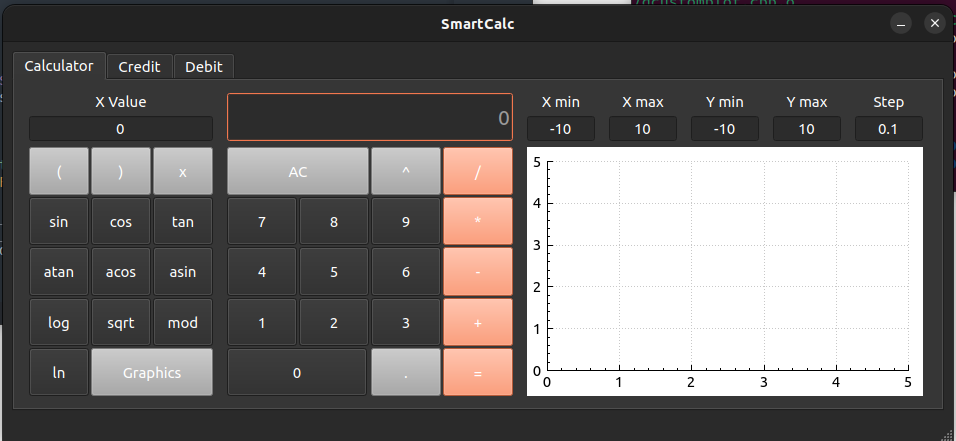
\includegraphics[width=15cm]{1}
	\par По умолчанию открывается вкладка Calculator, на которой можно:
	\begin{enumerate}		
		\item Вычислять бинарные операции: +, *, -, mod, /,\verb!^!
		\item Вычислять унарные операции: sin, cos, tan, acos, asin, atan, sqrt, ln, log
		\item Вычислять выражение, содержащее переменную \textit{x}, задавая значения переменной.
		\item Строить график функции, задавая область определения и значения функции.
	\end{enumerate}
		
	\par Примеры работы приложения:
	
	\par 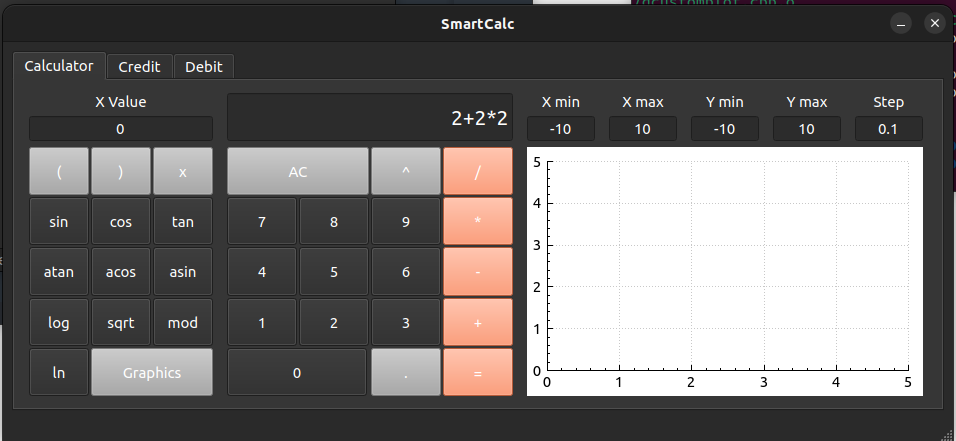
\includegraphics[width=12cm]{2}
	\par 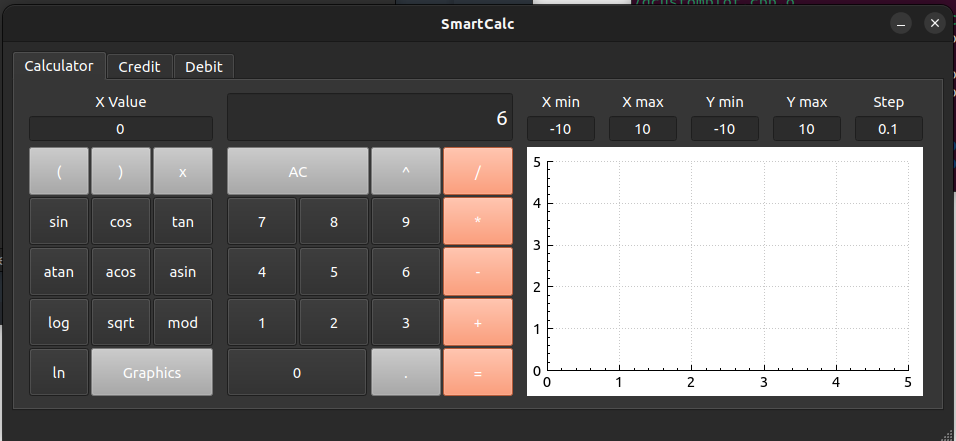
\includegraphics[width=12cm]{3}
	
	\par При вводе некорректного выражения, появится окно об ошибке \textit{INVALID EXPRESSION} :
	\par 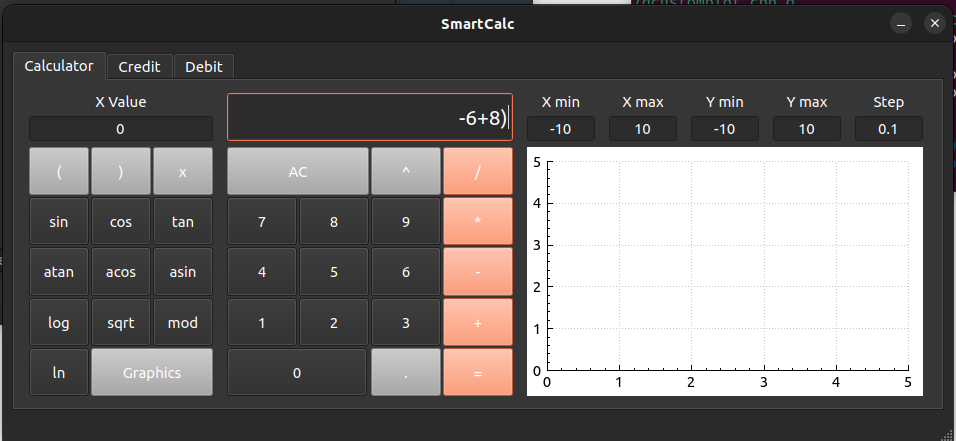
\includegraphics[width=12cm]{4}
	\par 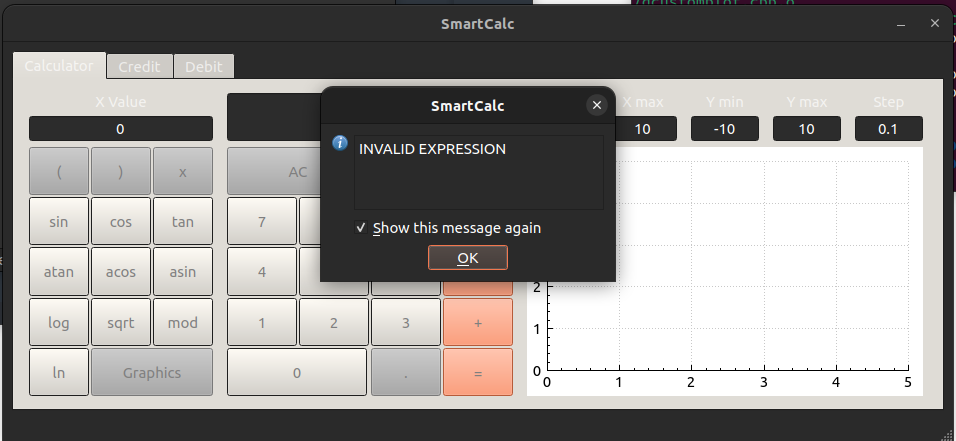
\includegraphics[width=12cm]{5}
	
	\par При вводе выражения c арифметическими ошибками, появится соответствующее окно об ошибке \textit{ERROR IN CALCULATION} :
	\par 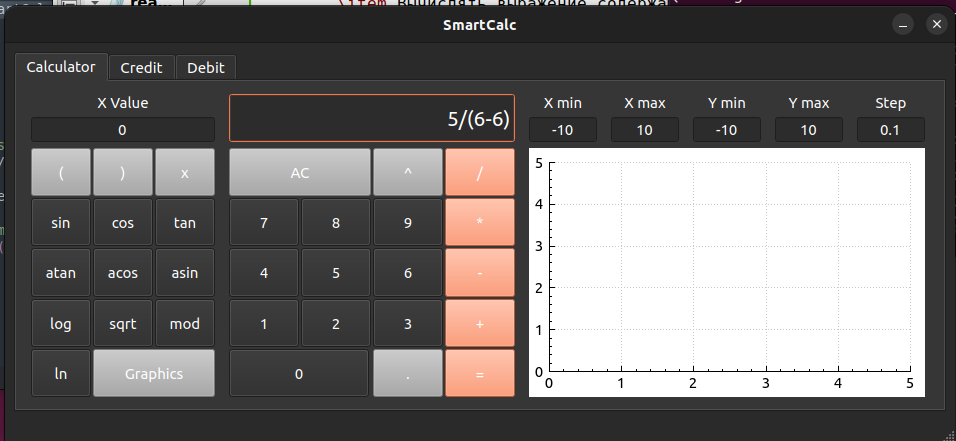
\includegraphics[width=12cm]{17}
	\par 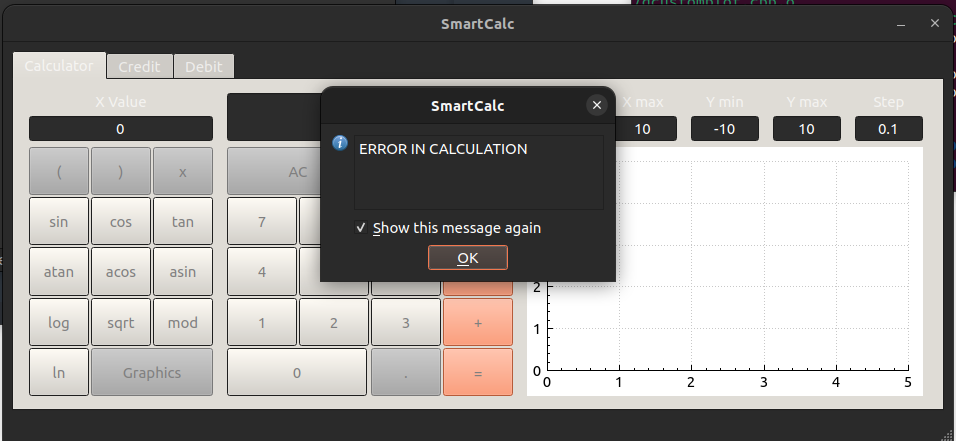
\includegraphics[width=12cm]{6}
	\centering
	\par При вводе выражения c переменной \textit{x}, можно ввести значение переменной под надписью \textit{X Value}:
	\par 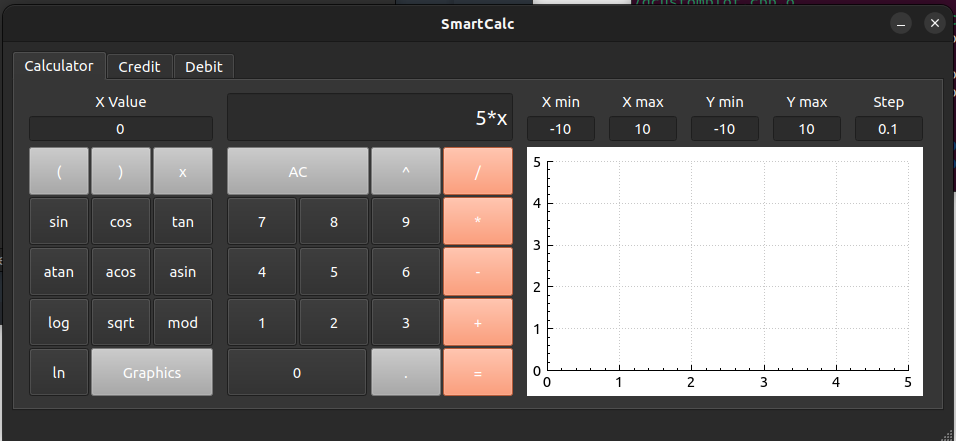
\includegraphics[width=12cm]{7}
	\par 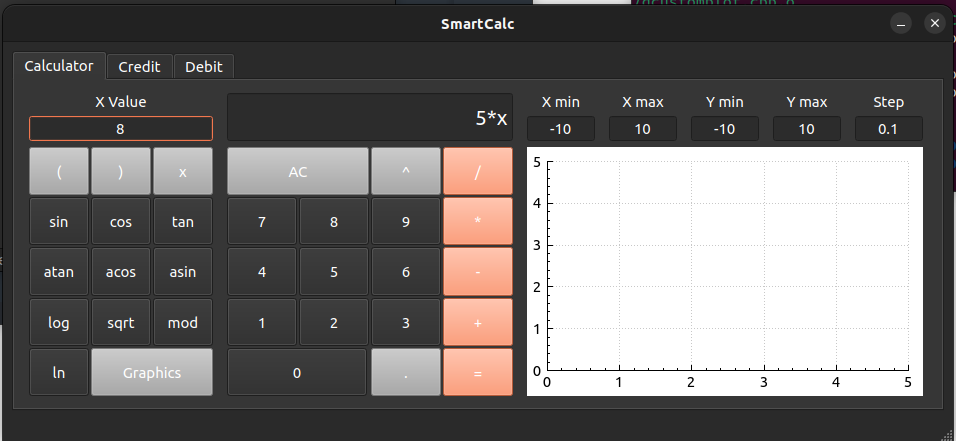
\includegraphics[width=12cm]{8}
	\par 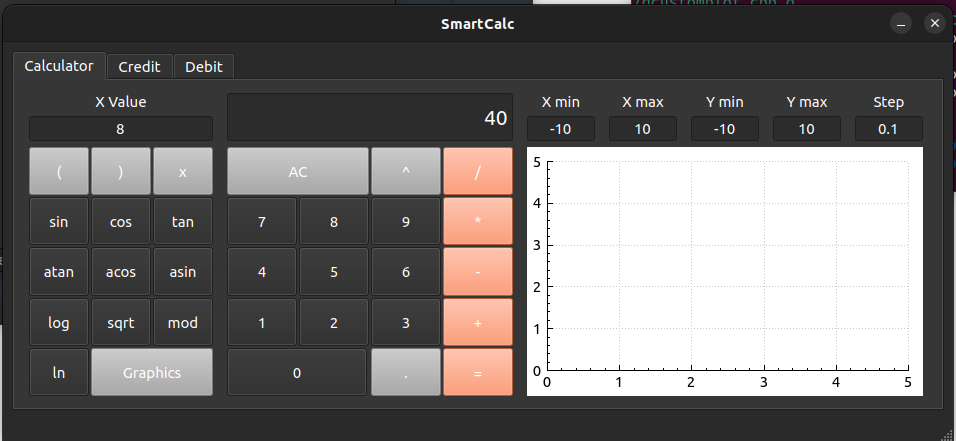
\includegraphics[width=12cm]{9}
	
	\par При вводе выражения c переменной \textit{x} и неккоректном значении переменной под надписью \textit{X Value}, повится окно об ошибке \textit{INVALID X VALUE} :
	\par 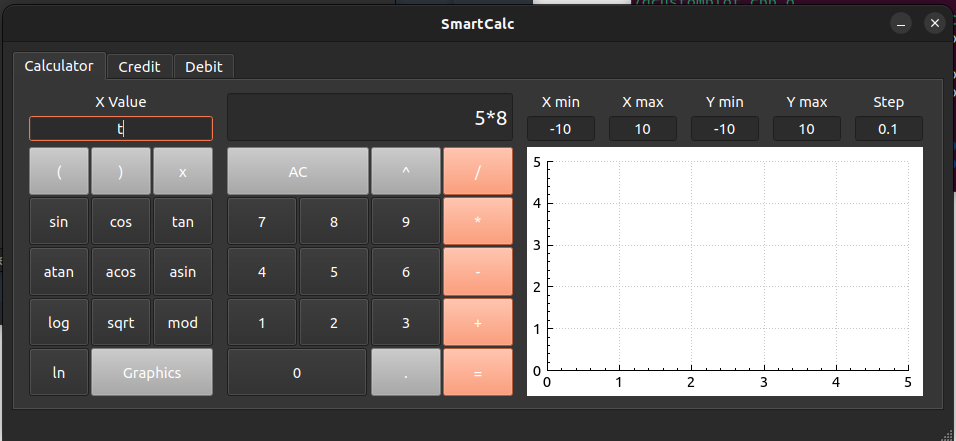
\includegraphics[width=12cm]{10}
	\par 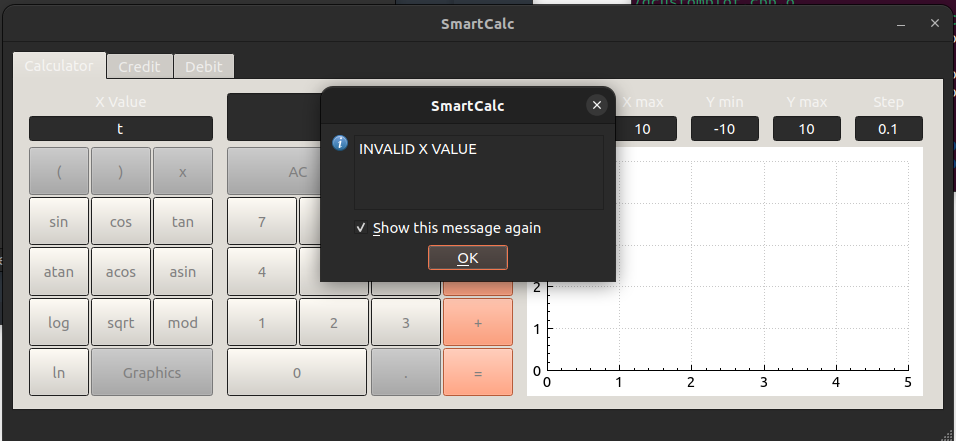
\includegraphics[width=12cm]{11}
	
	\par Построения графиков функций с разными границами области определения и значения функции:
	\par 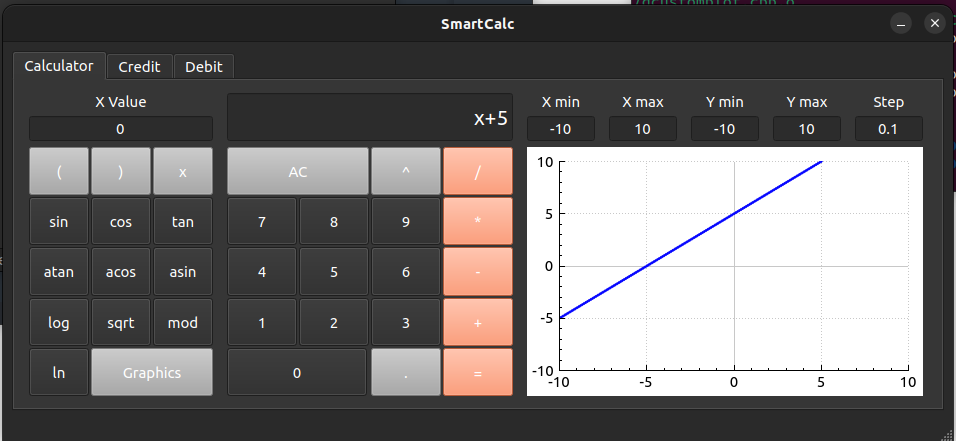
\includegraphics[width=12cm]{12}
	\par 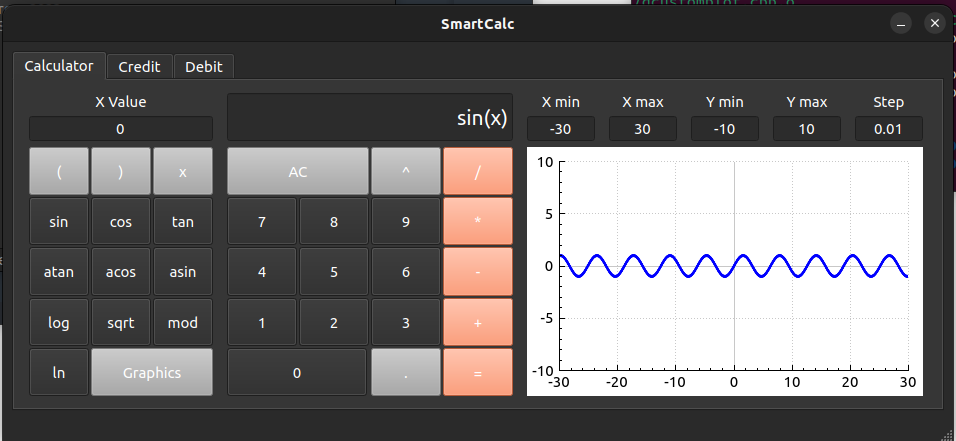
\includegraphics[width=12cm]{13}	

	\section{Credit}
	\begin{center}
		Вкладка \textit{Credit} предназначена для расчетов:
		\begin{itemize}
			\item Ежемесячного платежа
			\item Переплаты по кредиту
			\item Общей выплаты
		\end{itemize}
		
		\par Можно рассчитать по аннуитетному типу:
			\centering
			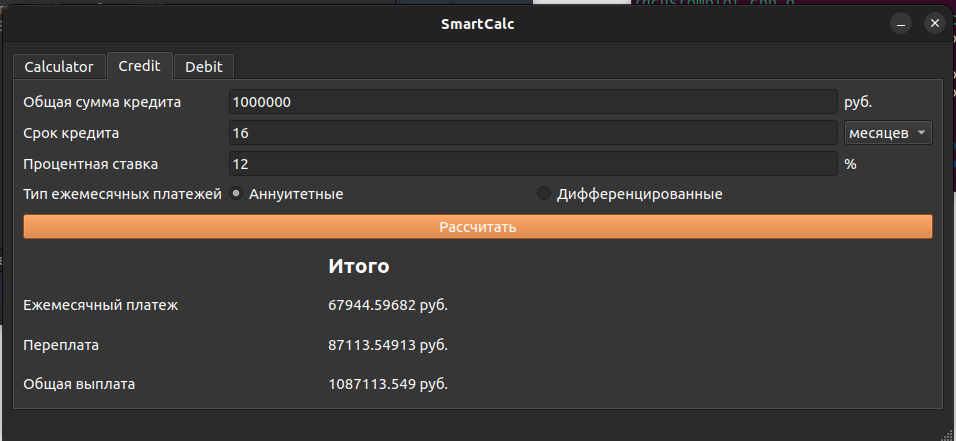
\includegraphics[width=12cm]{14}
		\par 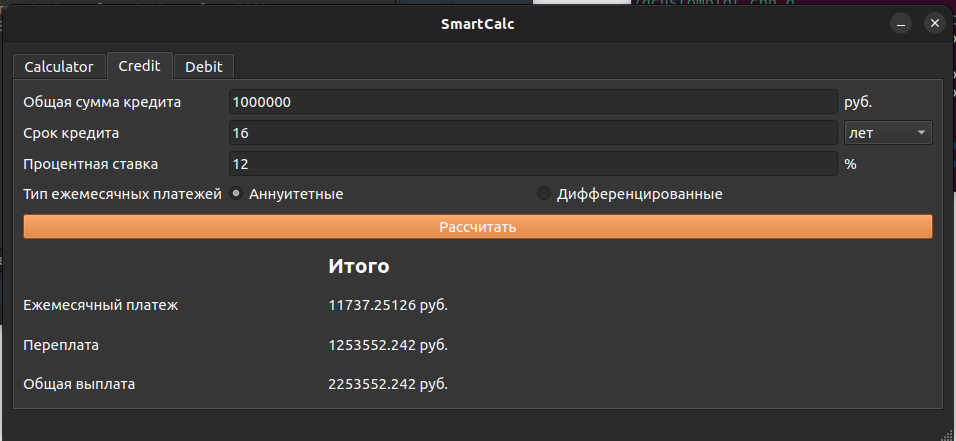
\includegraphics[width=12cm]{15}
		
		\par Можно рассчитать по дифференцированному типу:
			\centering
		\par 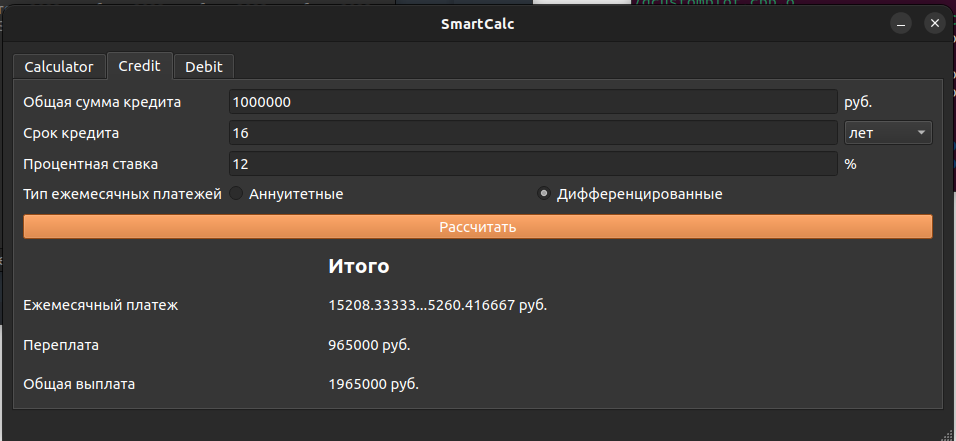
\includegraphics[width=12cm]{16}
	\end{center}	

	\section{Debit}
		Вкладка \textit{Debit} предназначена для расчетов:
	\begin{itemize}
		\item Начисленных процентов
		\item Суммы налога
		\item Суммы на вкладе к концу срока
	\end{itemize}
%	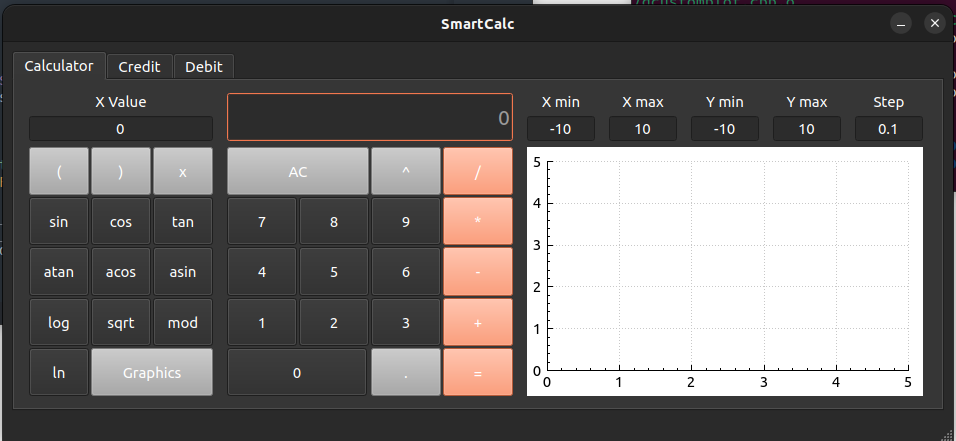
\includegraphics{1}
	
\end{document}